\frame{
\frametitle{Servidores de repositorios Git}

%Con Git instalado en nuestro computador tendremos un control de versiones con toda la funcionalidad, pero si nuestro proposito es compartir el c\'odigo con otras personas, debemos crear un repositorio en un servidor.

Algunos de ellos son:
\begin{itemize}
\item GitHub (Lo veremos m\'as detallado)
\item BitBucket
\item GitLab
\item Cloud Source Repositories (Beta)
\end{itemize}

\begin{figure}[t]
    \centering
    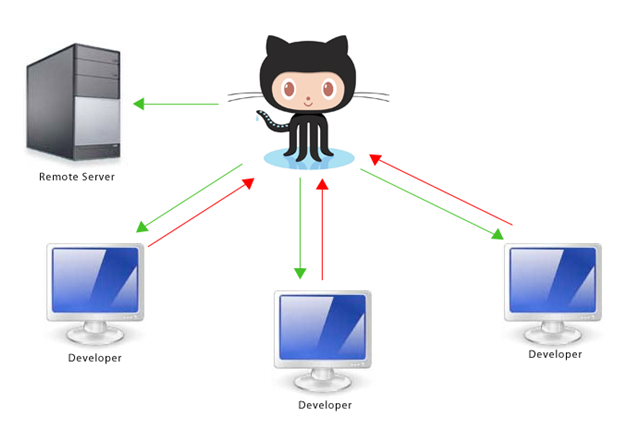
\includegraphics[width=0.5\textwidth]{Images/2}
\end{figure}

}
